% DOCUMENT CLASS SETUP
\documentclass[12pt, a4paper]{article}

% DOCUMENT PACKAGES
\usepackage[a4paper, margin=1in]{geometry}
\usepackage{titling}
\usepackage{enumitem}
\usepackage{amsmath}
\usepackage{amssymb}
\usepackage{mathtools}
\usepackage{graphicx}
\usepackage{xcolor}
\usepackage{listings}
\usepackage{hyperref}
\usepackage{csquotes}
\usepackage{tocloft}

% FONT AND ENCODING SETUP
\usepackage{fontspec}
\usepackage{polyglossia}
\usepackage[Thai]{ucharclasses}
\setdefaultlanguage{english}
\setotherlanguage{thai}
\setTransitionsFor{Thai}{\thaifont}{\normalfont}
\newfontfamily{\thaifont}{THSarabun.ttf}[
    Path=./,
    BoldFont=THSarabunBold.ttf,
    ItalicFont=THSarabunItalic.ttf,
    BoldItalicFont=THSarabunBoldItalic.ttf,
    Scale=1.23
]
\XeTeXlinebreaklocale "th"
\XeTeXlinebreakskip = 0pt plus 1pt

% PROFESSIONAL CODE BLOCK
\usepackage{tcolorbox}
\tcbuselibrary{minted, skins, breakable}

% DEFINE GITHUB DARK THEME COLORS %
\definecolor{ghback}{HTML}{0d1117}    % Dark background
\definecolor{ghtext}{HTML}{c9d1d9}    % Light gray text
\definecolor{ghborder}{HTML}{30363d}  % GitHub Border color

% PROFESSIONAL CODE BLOCK CONFIGURATION (MINTED VERSION) %
\renewcommand{\theFancyVerbLine}{\textcolor{white!60!gray}{\scriptsize\arabic{FancyVerbLine}}}
\newtcblisting{codeblock}[2][]{
    enhanced,
    breakable,
    colback=ghback,
    colframe=ghborder,
    coltitle=ghtext,
    colupper=ghtext,
    fonttitle=\bfseries\small,
    arc=3mm,
    boxrule=0.5mm,
    % PADDING SETTINGS
    left=25pt,
    right=10pt,
    top=5pt,
    bottom=5pt,
    % MINTED SETTINGS
    listing engine=minted,
    listing only,
    minted language=python,
    minted options={
        linenos,
        numbersep=5pt,
        fontsize=\footnotesize,
        breaklines=true,
        breakanywhere=true,
        autogobble,
        style=monokai,
    },
    title={#2},
    #1
}

% DOCUMENT TITLE SETUP %
\title {
	\textbf{2110446 DATA SCIENCE AND DATA ENGINEERING} \\
    \vspace{1em}
	\Large{\textbf{Take-Home Midterm Exam: Traffy Fondue}} \\
    \vspace{0.5em}
    \large{Computer Engineering, Chulalongkorn University}
}
\author{Worralop Srichainont}
\date{\today}
\setlength{\droptitle}{15em}

% DISABLE PAGE NUMBER IN TABLE OF CONTENTS
\tocloftpagestyle{empty}

% DOCUMENT CONTENTS
\begin{document}

    \maketitle
    \thispagestyle{empty}
    \clearpage

    \pagestyle{empty}
    \tableofcontents
    \clearpage

    \pagestyle{plain}
    \pagenumbering{arabic}

    \part{Introduction}
        \section{Traffy Fondue}
            \textbf{Traffy Fondue} is a digital platform developed by Thailand's National Electronics and Computer Technology (NECTEC)
            which allows residents to report infrastructure issues such as broken streetlights, garbage or flooding.

            \vspace{1em}

            It is adopted by the Bangkok Metropolitan Administration (BMA) as a central digital platform for the residents
            to report their issue and uses Artificial Intelligence (AI) to automatically send to the correct government department.
            The residents can access the service via LINE messaging app and a website.
            After reporting the issues, users receive updates on the progress.

            \vspace{1em}

            In March 2026, Bangkok Traffy Fondue has received more than 1,200,000 reports and more than 1,000,000 reports resolved.
            This shows that the system clearly improves efficiency, transparency, and citizen engagement of Bangkok government workflow.

        \section{Project Overview}
            This project focuses on building a pipeline to perform data preprocessing and implement machine learning model
            to classify the input report text according to government department below.
            \begin{enumerate}
                \item สำนักงานตำรวจแห่งชาติ
                \item การรถไฟฟ้าขนส่งมวลชนแห่งประเทศไทย
                \item สภาเด็กและเยาวชนกรุงเทพมหานคร
                \item กรมควบคุมมลพิษ
                \item กรมสรรพสามิต
                \item การไฟฟ้านครหลวง
                \item กรมทางหลวง
                \item สำนักงานประกันสุขภาพแห่งชาติ
                \item การประปานครหลวง
                \item คณะกรรมการการพัฒนาเศรษฐกิจ
                \item กระทรวงการท่องเที่ยวและกีฬา
                \item สำนักงาน กสทช. ศูนย์รับแจ้งปัญหา 1200
            \end{enumerate}

            Overall, this project uses \textbf{PyThaiNLP} for data preprocessing, \textbf{PhayaThaiBERT} for deep learning model
            and use \textbf{Macro F1 score} for evaluation.

    \pagebreak

        \section{Resources Links}

            \begin{table}[h]
                \centering
                \begin{tabular}{|l|c|}
                    \hline
                    \rule{0pt}{2.5ex}
                    \textbf{Resource} & \textbf{Link} \\
                    \hline \hline
                    Kaggle Dataset & \href{https://www.kaggle.com/datasets/worralopsrichainont/2110446-dsde-midterm-dataset-cleaned}{Link} \\
                    Raw Train Dataset & \href{https://drive.google.com/uc?id=1viyCPfSO-3vCwEpEfS6KhinpFk9_Ozg2}{Link} \\
                    Raw Test Dataset & \href{https://drive.google.com/uc?id=1o0redlOH2bDN8iZqqBZVew7Bb80KIeXo}{Link} \\
                    Cleaned Train Dataset & \href{https://drive.google.com/uc?id=1b_UK7477inZgaCib2oH8pniF9R8EkIWU}{Link} \\
                    Cleaned Test Dataset & \href{https://drive.google.com/uc?id=1DIaNv7YWiFKhTSoSvaBZ4YRudal-3m51}{Link} \\
                    Model Checkpoint & \href{https://drive.google.com/uc?id=1twq0FrPmmeP9nU0m4JWdJGUOp-SwXCWF}{Link} \\
                    Data Preprocessing Notebook & \href{https://www.kaggle.com/code/worralopsrichainont/2110446-dsde-midterm-preprocess}{Link} \\
                    EDA Notebook & \href{https://www.kaggle.com/code/worralopsrichainont/2110446-dsde-midterm-eda}{Link} \\
                    Model Notebook & \href{https://www.kaggle.com/code/worralopsrichainont/2110446-dsde-midterm-model}{Link} \\
                    \hline
                \end{tabular}
                \caption{Resources Link}
            \end{table}

    \pagebreak

    \part{Data Preparation}
        \section{Dependencies}
            Since the Kaggle Notebook or Google Colab Notebook environment doesn't have PyThaiNLP
            and Iterative Stratification library, we need to install the library using \texttt{pip}.
            \begin{codeblock}[minted language=bat]{Install Libraries}
                pip -q install pythainlp python-crfsuite
                pip install -U iterative-stratification
            \end{codeblock}

            \noindent Then import these libraries to perform the data preprocessing.
            \begin{itemize}
                \item \texttt{re} is for searching, matching and replace text in Python.
                \item \texttt{numpy} is for data array for data splitting.
                \item \texttt{pandas} is for tabular data manipulation.
                \item \texttt{tqdm} is for visualizing progress bar.
                \item \texttt{pythainlp} is for manipulating Thai text.
                \begin{itemize}
                    \item \texttt{normalize} is for reorder the Thai alphabet of every Thai text to the same standard.
                    \item \texttt{ThaiTextProcessor} is for creating the text processor object of PyThaiNLP.
                \end{itemize}
                \item \texttt{MultilabelStratifiedShuffleSplit} is for applying stratification for multi-label data splitting.
            \end{itemize}

            \begin{codeblock}{Dependencies}
                import re
                import numpy as np
                import pandas as pd

                from tqdm import tqdm
                from pythainlp.util import normalize
                from pythainlp.phayathaibert import ThaiTextProcessor
                from iterstrat.ml_stratifiers import MultilabelStratifiedShuffleSplit
            \end{codeblock}

    \pagebreak

        \section{Load Dataset}
            In the project, I have create the Traffy Fondue dataset in Kaggle which can be accessed by this link:
            \href{https://www.kaggle.com/datasets/worralopsrichainont/2110446-dsde-midterm-dataset-cleaned}{Kaggle Dataset}

            \vspace{0.5em}

            After adding Kaggle dataset into the Kaggle notebook, load the dataset using the pandas command.

            \begin{codeblock}{Load Dataset}
                TRAIN_FILE_PATH = "/kaggle/input/datasets/worralopsrichainont/2110446-dsde-midterm-dataset-cleaned/train.csv"
                TEST_FILE_PATH = "/kaggle/input/datasets/worralopsrichainont/2110446-dsde-midterm-dataset-cleaned/test.csv"

                df_train = pd.read_csv(TRAIN_FILE_PATH)
                df_test = pd.read_csv(TEST_FILE_PATH)
            \end{codeblock}

        \section{Data Cleaning}
            \subsection{Regex Pattern}
                To make the regex operation easier to debug, create a pattern constant for each category.
                \begin{itemize}
                    \item \textbf{HTML Pattern} use to find and match any tags inside \texttt{<>} tags (e.g. \texttt{<body>}) in the text.
                    \item \textbf{Phone Pattern} use to find and match Thai telephone number in the text.
                    \begin{itemize}
                        \item \textbf{Thai Mobile Number}: Telephone number with 10 digits starts with 06 or 08 or 09
                        \item \textbf{Thai Landlines Number}: Telephone number with 9 digits starts with 02 or 03 or 04 or 09
                        \item \textbf{Thai Toll-free Number}: Telephone number with 10 digits starts with 1800 or 1900 or 1401
                        \item \textbf{Thai Hotlines}: 1555, 1129, 1125, 1137, 1644, 1669, 191, 199
                    \end{itemize}
                    \item \textbf{Email Pattern} use to find and match any email in the text.
                    \item \textbf{URL Pattern} use to find any URL in the text.
                    \item \textbf{Zero Width Pattern} use to find any zero width characters.
                    \item \textbf{Whitelist Character Pattern} use to filter only Thai characters, English characters
                    digits, some punctuations and spaces.
                    \item \textbf{Whitespace Pattern}: use to convert newline spaces and tab spaces to spaces.
                \end{itemize}

    \pagebreak

                \begin{codeblock}{Regex Pattern}
                    HTML_PATTERN = re.compile(r"<[^<>]*>")

                    PHONE_PATTERN = re.compile(
                        r"(?<![\d/.:])(?:"
                        r"0[689]\d[- ]?\d{3}[- ]?\d{4}|"
                        r"02[- ]?\d{3}[- ]?\d{4}|"
                        r"0[3457]\d[- ]?\d{3}[- ]?\d{3}|"
                        r"(?:1800|1900|1401)[- ]?\d{3}[- ]?\d{3}|"
                        r"1555|1129|1125|1137|1644|1669|191|199"
                        r")(?![\d/.:])"
                    )

                    EMAIL_PATTERN = re.compile(r"[a-zA-Z0-9_.+-]+@[a-zA-Z0-9-]+\.[a-zA-Z0-9-.]+")

                    URL_PATTERN = re.compile(r"https?://[^\s\u0E01-\u0E5B]+|www\.[^\s\u0E01-\u0E5B]+")

                    ZERO_WIDTH_CHARS_PATTERN = re.compile(r"[\u200B\u200C\u200D\uFEFF]+")

                    PUNCTUATION_PATTERN = re.compile(r'([!"\'(),./:;?#-])\1+')

                    ALLOWED_PUNC = r"""!"'(),./:;?#-"""
                    WHITELIST_PATTERN = re.compile(rf"[^a-zA-Z0-9\u0E01-\u0E5B\s{re.escape(ALLOWED_PUNC)}฿]")

                    WHITESPACE_PATTERN = re.compile(r"\s+")
                \end{codeblock}

    \pagebreak

            \subsection{Defining Class}
                The Thai text cleaning process is as follows
                \begin{enumerate}
                    \item Convert all English characters to the lowercase and remove trailing spaces.
                    \item Remove HTML tags.
                    \item Remove telephone number.
                    \item Remove email.
                    \item Remove URL.
                    \item Remove zero width characters.
                    \item Remove all characters that is not Thai characters, English characters, digits,
                    some punctuations and space.
                    \item Convert all tab space (\texttt{"\textbackslash t"}) and newline space (\texttt{"\textbackslash n"}) to space (\texttt{" "}).
                    \item Add space between \texttt{\#} and its content (e.g. \texttt{\#traffyfondue} $\rightarrow$ \texttt{\# traffyfondue})
                    \item Reorder all Thai characters of the text to the same standard.
                    \item Remove redundant characters (e.g. convert รอนานมากกกกกกกก to รอนานมาก)
                \end{enumerate}

            \begin{codeblock}{Text Cleaner Class}
                class TextCleanerBERT:
                    THAI_TEXT_PROCESSOR = ThaiTextProcessor()

                    @staticmethod
                    def get_cleaned_thai_text(text):
                        if not isinstance(text, str):
                            return text

                        text = text.lower().strip()
                        text = TextCleanerBERT.remove_html(text)
                        text = TextCleanerBERT.remove_telephone_number(text)
                        text = TextCleanerBERT.remove_email(text)
                        text = TextCleanerBERT.remove_url(text)
                        text = TextCleanerBERT.remove_zero_width_chars(text)
                        text = TextCleanerBERT.remove_non_whitelist_chars(text)
                        text = TextCleanerBERT.clean_punctuation(text)
                        text = TextCleanerBERT.pad_hashtags(text)

                        text = normalize(text)
                        text = TextCleanerBERT.remove_redundant_chars(text)
                        text = TextCleanerBERT.clean_whitespace(text)
                        return text

                    @staticmethod
                    def remove_html(text):
                        return HTML_PATTERN.sub("", text)

                    @staticmethod
                    def remove_telephone_number(text):
                        return PHONE_PATTERN.sub("", text)

                    @staticmethod
                    def remove_email(text):
                        return EMAIL_PATTERN.sub("", text)

                    @staticmethod
                    def remove_url(text):
                        return URL_PATTERN.sub("", text)

                    @staticmethod
                    def remove_zero_width_chars(text):
                        return ZERO_WIDTH_CHARS_PATTERN.sub("", text)

                    @staticmethod
                    def remove_non_whitelist_chars(text):
                        return WHITELIST_PATTERN.sub(" ", text)

                    @staticmethod
                    def clean_punctuation(text):
                        return PUNCTUATION_PATTERN.sub(r"\1", text)

                    @staticmethod
                    def pad_hashtags(text):
                        return text.replace("#", " # ")

                    @staticmethod
                    def remove_redundant_chars(text):
                        return TextCleanerBERT.THAI_TEXT_PROCESSOR.replace_rep_after(text)

                    @staticmethod
                    def clean_whitespace(text):
                        text = WHITESPACE_PATTERN.sub(" ", text)
                        return text.strip()
            \end{codeblock}

            \subsection{Data Cleaning}
                Do the following operations to clean the dataset
                \begin{enumerate}
                    \item Remove all rows with missing value by using \texttt{dropna()}.
                    \item Apply text cleaning function of train dataset.
                    \item Apply text cleaning function of test dataset.
                \end{enumerate}

                \begin{codeblock}{Data Cleaning}
                    df_train = df_train.dropna()

                    tqdm.pandas(desc="Cleaning Train Dataset")
                    df_train["comment"] = df_train["comment"].progress_apply(
                        TextCleanerBERT.get_cleaned_thai_text
                    )
                    tqdm.pandas(desc="Cleaning Test Dataset")
                    df_test["comment"] = df_test["comment"].progress_apply(
                        TextCleanerBERT.get_cleaned_thai_text
                    )
                \end{codeblock}

    \pagebreak

        \section{Data Splitting}
            Now, we are going to perform the splitting all data rows in \texttt{train.csv} into train dataset
            and validation dataset by using stratification to ensure the class ratio in both dataset.

            \vspace{0.5em}

            All rows in the file \texttt{train.csv} has 304,284 rows and 14 columns
            (including \texttt{id}, \texttt{comment} and other 12 categorical columns)
            \begin{itemize}
                \item \textbf{Train Dataset} used for training the model which has 273,855 rows and 14 columns (90\% of data)
                \item \textbf{Validation Dataset} used for tuning the model hyper-parameters which has 30,429 rows and 14 columns (10\% of data)
            \end{itemize}

            \begin{codeblock}{Configuration}
                VALIDATION_DATASET_RATIO = 0.1
                SEED = 42

                TEXT_COL = "comment"

                LABEL_COLS = [
                    "สำนักงานตำรวจแห่งชาติ",
                    "การรถไฟฟ้าขนส่งมวลชนแห่งประเทศไทย",
                    "สภาเด็กและเยาวชนกรุงเทพมหานคร",
                    "กรมควบคุมมลพิษ",
                    "กรมสรรพสามิต",
                    "การไฟฟ้านครหลวง",
                    "กรมทางหลวง",
                    "สำนักงานประกันสุขภาพแห่งชาติ",
                    "การประปานครหลวง",
                    "คณะกรรมการการพัฒนาเศรษฐกิจ",
                    "กระทรวงการท่องเที่ยวและกีฬา",
                    "สำนักงาน กสทช. ศูนย์รับแจ้งปัญหา 1200",
                ]
            \end{codeblock}

            \noindent First, Extract feature and label columns from the dataset.
            \begin{codeblock}{Extract Feature and Label}
                X = df_train_all['comment'].to_numpy()
                y = df_train_all[LABEL_COLS].to_numpy()
            \end{codeblock}

            \noindent Then, split the dataset using the multi-label stratification.
            \begin{codeblock}{Multi-label Stratification}
                # Create a multi-label dataset splitter
                msss = MultilabelStratifiedShuffleSplit(
                    n_splits=1,
                    test_size=VALIDATION_DATASET_RATIO,
                    random_state=SEED
                )
                # Begin dataset splitting
                for train_index, val_index in msss.split(X, y):
                    df_train = df_train_all.iloc[train_index].reset_index(drop=True)
                    df_val = df_train_all.iloc[val_index].reset_index(drop=True)
            \end{codeblock}

    \pagebreak

        \section{PyTorch DataLoader}
            \subsection{Dependencies}
                After splitting train dataset and validation dataset in \texttt{pandas},
                we need to create PyTorch DataLoader to properly feed data as a batch to the PyTorch model.

                \vspace{0.5em}

                However, the Kaggle Notebook or Google Colab Notebook environment doesn't have transformer model library
                PyTorchLightning framework, we need to install the framework using \texttt{pip}.

                \begin{codeblock}[minted language=bat]{Install Libraries and Frameworks}
                    pip install -U lightning
                    pip install -U transformer
                \end{codeblock}

                \noindent Then import these libraries to create the PyTorch DataLoader.
                \begin{itemize}
                    \item \texttt{torch} is for create and implement deep learning model.
                    \item \texttt{pytorch\_lightning} is a framework for organize the model code.
                    \item \texttt{Dataset} is for converting pandas dataframe into PyTorch dataset.
                    \item \texttt{DataLoader} is for creating a wrapper for PyTorch Dataset which can
                    send data as a batch to the PyTorch deep learning model.
                    \item \texttt{AutoTokenizer} is for encoding Thai text for PhayaThaiBERT model.
                \end{itemize}

                \begin{codeblock}{Dependencies}
                    import torch
                    import pytorch_lightning as pl
                    from torch.utils.data import Dataset, DataLoader
                    from transformers import AutoTokenizer
                \end{codeblock}

                To ensure the consistency of the result, we need to set the seed for every PyTorch operation.
                These are also including model section.
                \begin{codeblock}{Setup PyTorch Seed}
                    pl.seed_everything(42, workers=True)
                \end{codeblock}

    \pagebreak

            \subsection{Text AutoTokenizer}
                Before feeding the text into the PhayaThaiBERT deep learning model, we need to tokenize them first.
                In this section, we will loading the PhayaThaiBERT pre-trained model for a tokenizer.

                \begin{codeblock}{Tokenizer Configuration}
                    MODEL_NAME = "clicknext/phayathaibert"
                    MAX_LENGTH = 128
                    TEXT_COL = "comment"
                \end{codeblock}

                Now, we are going to implement the tokenizer from the PhayaThaiBERT pre-trained model.
                As for the maximum token length, we are choosing 128 tokens according to the EDA.

                \begin{codeblock}{Thai Text Tokenizer}
                    class ThaiTokenizer:
                        # Load pre-trained PhayaThaiBERT tokenizer
                        TOKENIZER = AutoTokenizer.from_pretrained(MODEL_NAME)

                        @staticmethod
                        def get_encoded_text(text):
                            # Encode text by using the tokenizer
                            encoded_text = ThaiTokenizer.TOKENIZER(
                                str(text),
                                max_length=MAX_LENGTH,
                                padding="max_length",
                                truncation=True,
                                add_special_tokens=True,
                                return_attention_mask=True,
                                return_tensors="pt",
                            )

                            # Return an encoded text
                            return encoded_text
                \end{codeblock}

    \pagebreak

            \subsection{PyTorch Dataset}
                After creating the PhayaThaiBERT tokenizer to encode the text, we need to create the PyTorch
                dataset for compatible with the PyTorch deep learning model.

                \begin{itemize}
                    \item \texttt{\_\_init\_\_} is the constructor method which contains
                    \begin{itemize}
                        \item \texttt{has\_label} is \texttt{True} for train dataset and validation dataset
                        but \texttt{False} for test dataset.
                        \item \texttt{texts} is the report text column as a numpy array.
                        \item \texttt{labels} is the label columns as a numpy array.
                        \item \texttt{n\_rows} is the rows amount of the dataset.
                    \end{itemize}
                    \item \texttt{\_\_len\_\_} returns the rows amount of the dataset.
                    \item \texttt{\_\_getitem\_\_} return the encoded text by the tokenizer of the index in the dataset
                    which return as a dict of \texttt{input\_ids}, \texttt{attention\_mask} and \texttt{labels}.
                \end{itemize}

                \begin{codeblock}{PyTorch Dataset}
                    class TraffyFondueDataset(Dataset):
                        def __init__(self, df, has_label):
                            # Store if the the dataset has label or not
                            self.has_label = has_label

                            # Separate text and label from a Pandas DataFrame
                            self.texts = df[TEXT_COL].to_numpy()
                            if self.has_label:
                                self.labels = df[LABEL_COLS].to_numpy(dtype=np.float32)

                            # Store rows amount of the dataset
                            self.n_rows = df.shape[0]

                        def __len__(self):
                            # Return length of the dataset
                            return self.n_rows

                        def __getitem__(self, idx):
                            # Encode the text using tokenizer
                            encoded_text = ThaiTokenizer.get_encoded_text(self.texts[idx])

                            # Return an item as a dict
                            item = {
                                "input_ids": encoded_text["input_ids"].squeeze(0),
                                "attention_mask": encoded_text["attention_mask"].squeeze(0),
                            }
                            if self.has_label:
                                item["labels"] = torch.tensor(self.labels[idx])

                            return item
                \end{codeblock}

    \pagebreak

            \subsection{PyTorch DataLoader}
                After creating the PyTorch dataset, we still require PyTorch DataLoader to easily feed multiple dataset rows
                as a batch to the PyTorch deep learning model. Here, we are going to set batch size to 32 to make this DataLoader
                feeds 32 rows to the deep learning model at once.

                \begin{codeblock}{DataLoader Configuration}
                    BATCH_SIZE = 32
                    NUM_WORKERS = 2
                \end{codeblock}

                Next, we are going to implement the PyTorch DataLoader as a class. In this part, it is the constructor method
                which initialize the batch size attribute, train dataset, validation dataset and test dataset.

                \begin{codeblock}{PyTorch DataLoader Constructor}
                    class TraffyFondueDataModule(pl.LightningDataModule):
                        def __init__(self, df_train, df_val, df_test):
                            super().__init__()
                            self.batch_size = BATCH_SIZE
                            self.num_workers = NUM_WORKERS

                            self.df_train = df_train
                            self.df_val = df_val
                            self.df_test = df_test
                \end{codeblock}

                Then, create the train PyTorch DataLoader from the train PyTorch Dataset.
                Make sure to set the \texttt{shuffle} to \texttt{True} for shuffling the order of data inside a batch
                to prevent a model to just memorize the data order pattern instead of actually understanding the context.
                \begin{codeblock}{Train DataLoader}
                    class TraffyFondueDataModule(pl.LightningDataModule):
                        def train_dataloader(self):
                            dataset_train = TraffyFondueDataset(self.df_train, True)

                            return DataLoader(
                                dataset_train,
                                batch_size=self.batch_size,
                                shuffle=True,
                                num_workers=self.num_workers,
                                pin_memory=True,
                            )
                \end{codeblock}

	\pagebreak

                Then, create the validation PyTorch DataLoader from the validation PyTorch Dataset.
                Set the \texttt{shuffle} to \texttt{False} because it is just for evaluation the model performance.
                \begin{codeblock}{Validation DataLoader}
                    class TraffyFondueDataModule(pl.LightningDataModule):
                        def val_dataloader(self):
                            dataset_val = TraffyFondueDataset(self.df_val, True)

                            return DataLoader(
                                dataset_val,
                                batch_size=self.batch_size,
                                shuffle=False,
                                num_workers=self.num_workers,
                                pin_memory=True,
                            )
                \end{codeblock}

                Then, create the test PyTorch DataLoader from the test PyTorch Dataset.
                Set the \texttt{shuffle} to \texttt{False} because it is just for evaluation the model performance.
                \begin{codeblock}{Test DataLoader}
                    class TraffyFondueDataModule(pl.LightningDataModule):
                        def test_dataloader(self):
                            dataset_test = TraffyFondueDataset(self.df_test, False)

                            return DataLoader(
                                dataset_test,
                                batch_size=self.batch_size,
                                shuffle=False,
                                num_workers=self.num_workers,
                                pin_memory=True,
                            )
                \end{codeblock}

    \pagebreak

        \section{Exploratory Data Analysis (EDA)}
            In this section, we are going to focus about plotting and finding insights from the dataset
            before training a deep learning model.

            \subsection{Class Count}
                \subsubsection{Visualization}
                    In this part, we are going to visualize the amount of classes from the dataset which is shown below.
                    \begin{figure}[h]
                        \centering
                        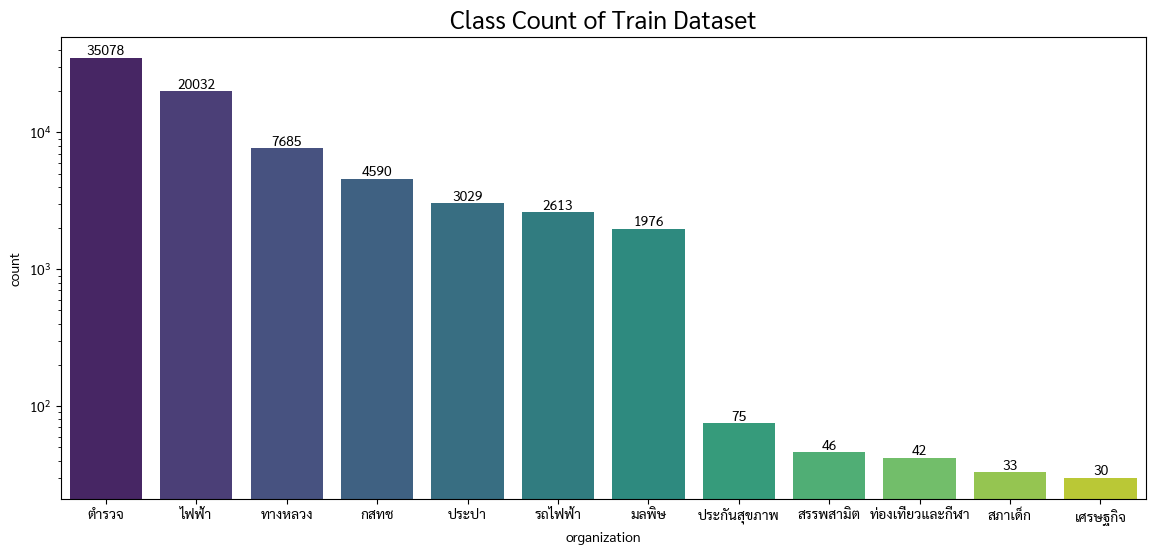
\includegraphics[width=\textwidth]{image_01}
                        \caption{Class Count}
                    \end{figure}

                \subsubsection{Insights}
                    The visualization shows that the dataset has extreme class imbalance and mostly are non-labeled data.
                    Therefore, we need to customize the penalty weight on model validation process to make the model
                    prioritize the minor classes too, not just the major classes.

                    \vspace{0.5em}

                    \noindent The data table is in the next page $\rightarrow$

    \pagebreak

                    \begin{table}[h]
                        \centering
                        \begin{tabular}{|l|c|c|}
                            \hline
                            \rule{0pt}{2.5ex}
                            \textbf{Organization} & \textbf{Count} & \textbf{Percentage} \\
                            \hline \hline
                            Non-labeled & 231,285 & 76.01\% \\
                            สำนักงานตำรวจแห่งชาติ & 35,078 & 11.53\% \\
                            การไฟฟ้านครหลวง & 20,032 & 6.58\% \\
                            กรมทางหลวง & 7,685 & 2.53\% \\
                            สำนักงาน กสทช. & 4,590 & 1.51\% \\
                            การประปานครหลวง & 3,029 & 1.00\% \\
                            การรถไฟฟ้าขนส่งมวลชน & 2,613 & 0.86\% \\
                            กรมควบคุมมลพิษ & 1,976 & 0.65\% \\
                            สำนักงานประกันสุขภาพ & 75 & 0.02\% \\
                            กรมสรรพสามิต & 46 & 0.02\% \\
                            กระทรวงการท่องเที่ยวและกีฬา & 42 & 0.01\% \\
                            สภาเด็กและเยาวชน & 33 & 0.01\% \\
                            คณะกรรมการการพัฒนาเศรษฐกิจ & 30 & 0.01\% \\
                            \hline
                        \end{tabular}
                        \caption{Class Count}
                    \end{table}

    \pagebreak

            \subsection{Label Cardinality}
                \subsubsection{Overall Visualization}
                    In this part, we are going to visualize the amount of rows in each label cardinality.
                    The label cardinality is the count of label of a single rows
                    (e.g. a row with สำนักงานตำรวจ and การไฟฟ้านครหลวง has label cardinality equals to 2)

                    \begin{figure}[h]
                        \centering
                        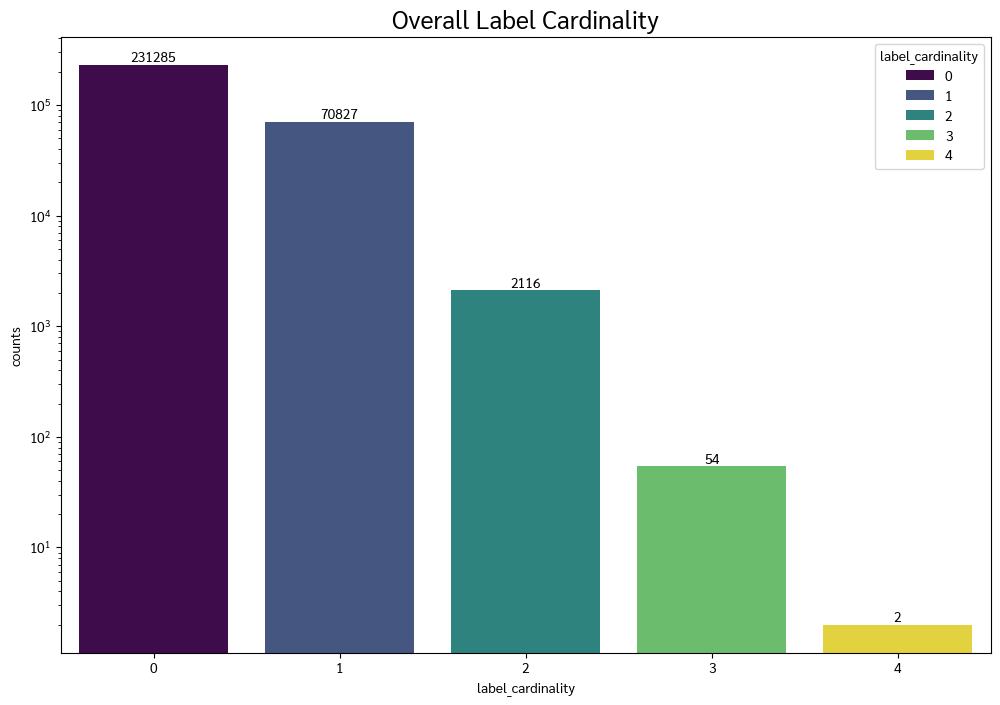
\includegraphics[width=\textwidth]{image_02}
                        \caption{Overall Label Cardinality}
                    \end{figure}

                \subsubsection{Categorical Visualization}
                    Next, we are going to visualize each label cardinality separated by classes
                    to identify which category likely has the multi-label.

                    \vspace{0.5em}

                    \noindent The visualization is in the next page $\rightarrow$

    \pagebreak

                    \begin{figure}[h]
                        \centering
                        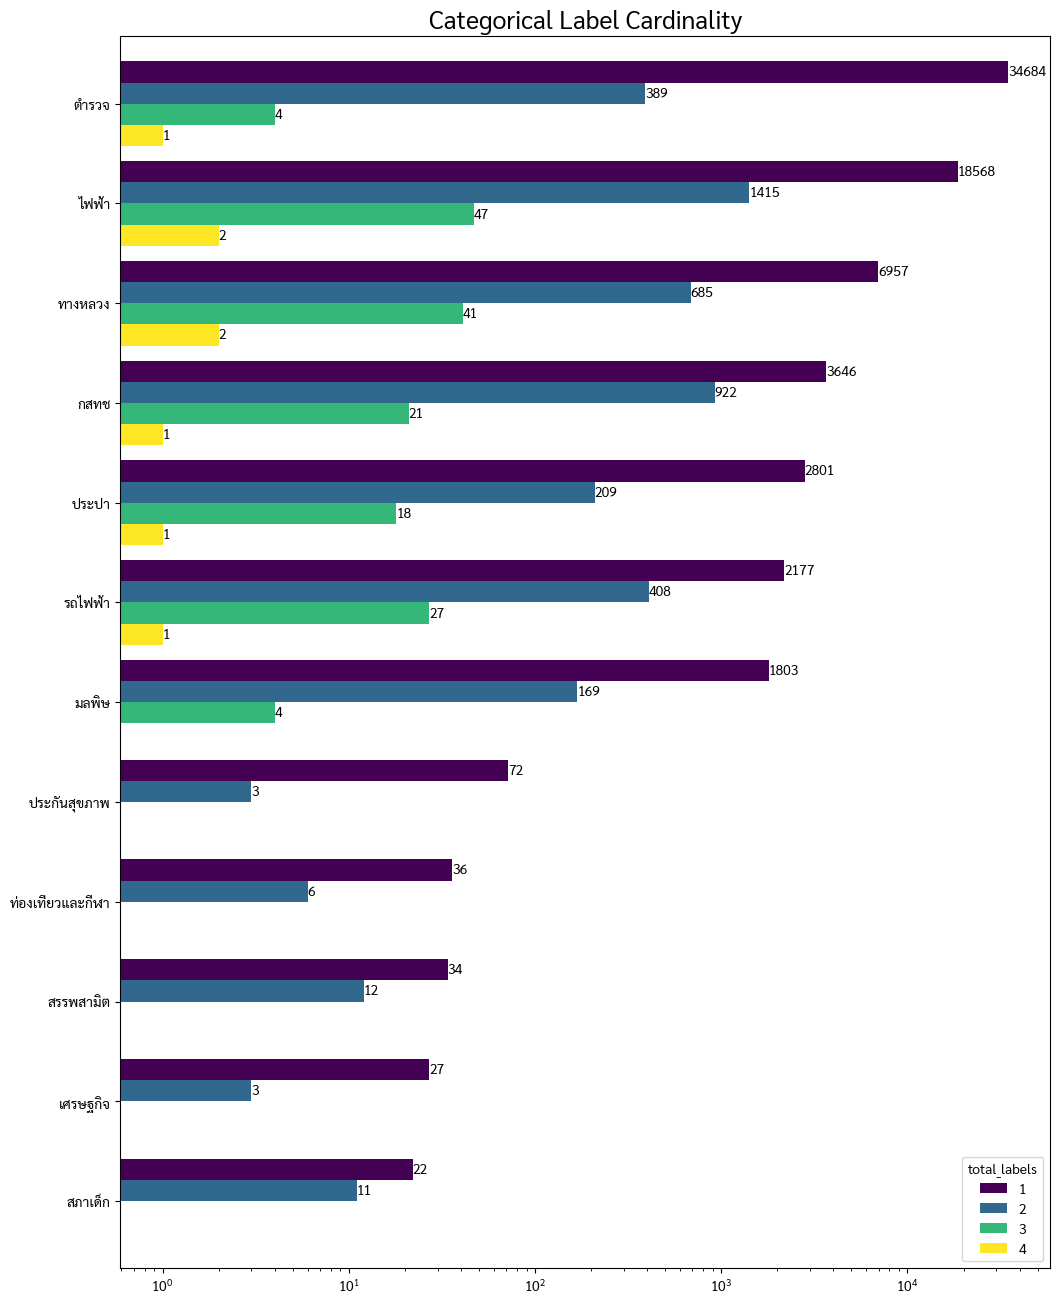
\includegraphics[width=0.9\textwidth]{image_03}
                        \caption{Categorical Label Cardinality}
                    \end{figure}

                \subsubsection{Insights}
                    The visualization shows that the dataset is mostly non-labeled with 231,285 rows.
                    In addition, the labeled data are mostly 1 label with 70,827 rows.
                    This shows that while most complaints belong to one organization,
                    the multi-label still exists so \textbf{BCEWithLogitsLoss} is the appropriate loss function for this task.

    \pagebreak

            \subsection{Co-occurrence Heatmap}
                \subsubsection{Visualization}
                    In this part, we are going to visualize the co-occurrence between the classes from the dataset which is shown below.

                    \begin{figure}[h]
                        \centering
                        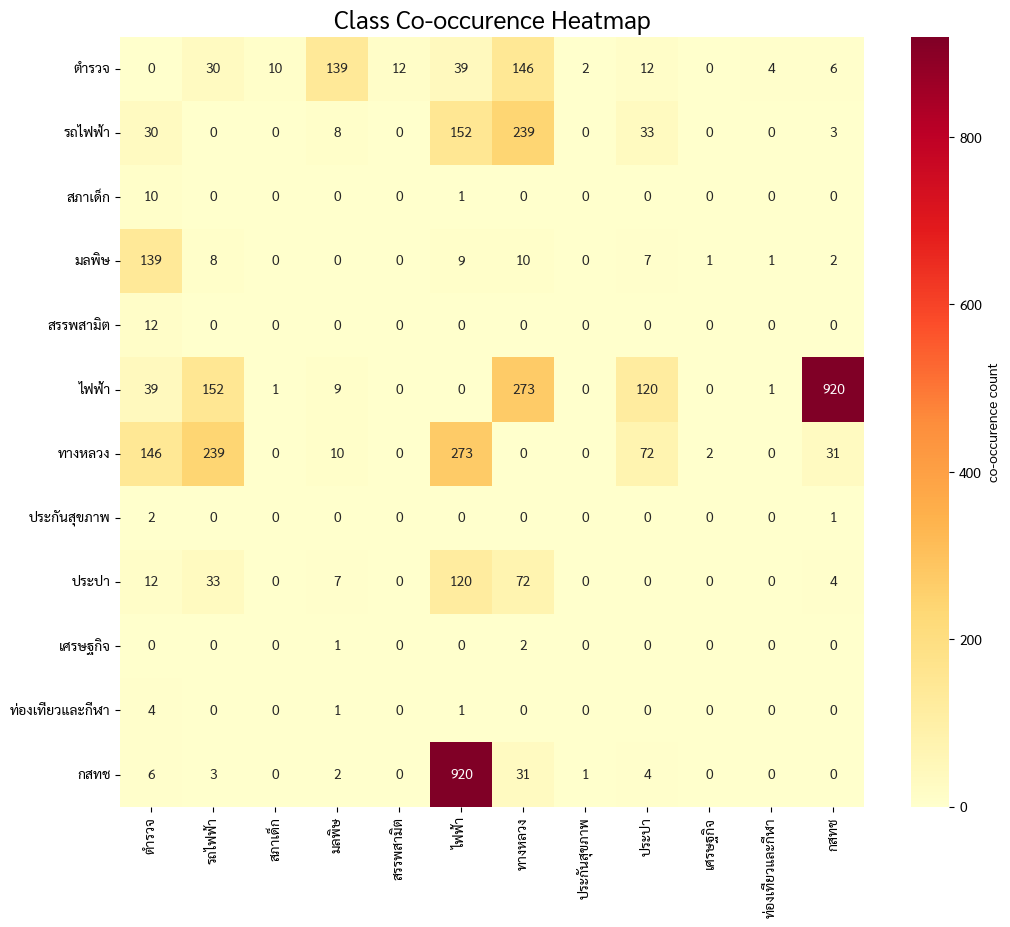
\includegraphics[width=\textwidth]{image_04}
                        \caption{Co-occurrence Heatmap}
                    \end{figure}

                \subsubsection{Insights}
                    The visualization shows that the การไฟฟ้านครหลวง organization and สำนักงาน กสทช has significant co-occurrence
                    with 920 cases. These two organizations may have interesting shared parts of the complaints.

    \pagebreak

            \subsection{Token Length Distribution}
                \subsubsection{Visualization}
                    In this part, we are going to visualize the token length distribution of the complaints from the dataset which is shown below.
                    \begin{figure}[h]
                        \centering
                        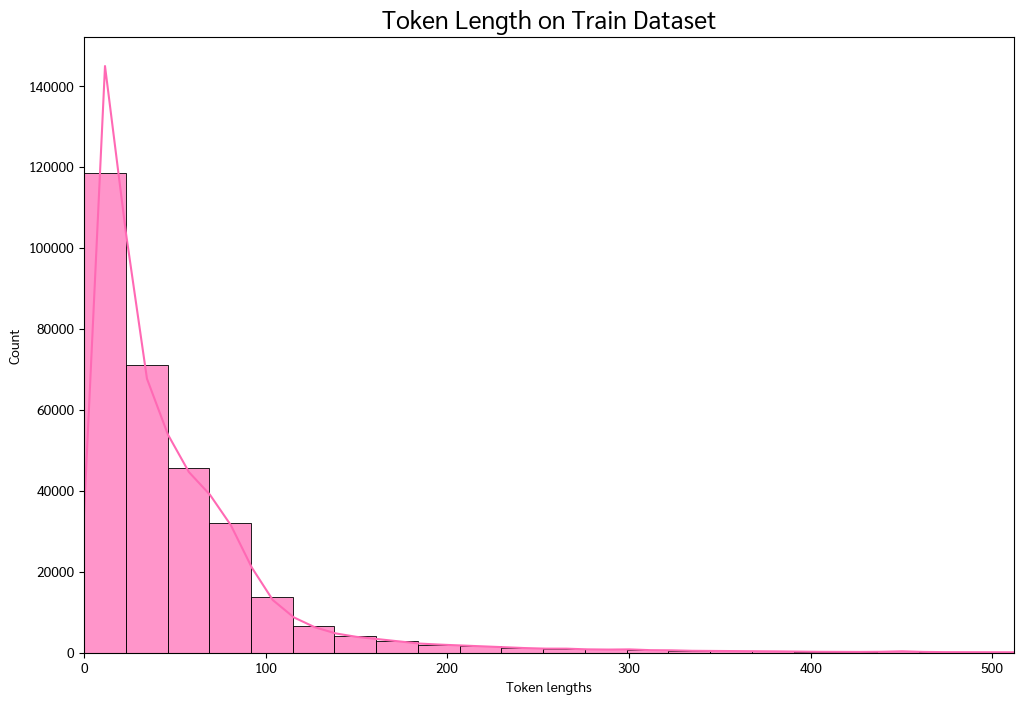
\includegraphics[width=0.7\textwidth]{image_05}
                        \caption{Train Dataset Token Length Distribution}
                    \end{figure}

                    \begin{figure}[h]
                        \centering
                        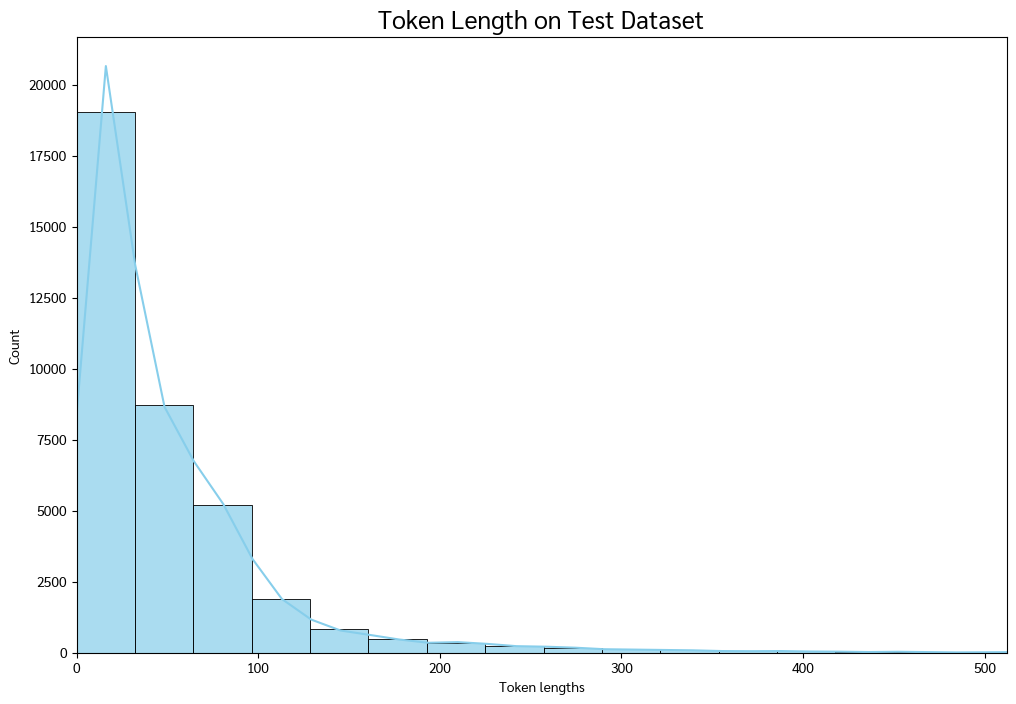
\includegraphics[width=0.7\textwidth]{image_06}
                        \caption{Test Dataset Token Length Distribution}
                    \end{figure}

    \pagebreak

                \subsubsection{Insights}
                    The visualization shows that the token length distribution of both train dataset and test dataset have
                    a similar distribution which is heavily right skew.
                    According to the table below, we should set the maximum token length on the data preparation to 128 tokens.

                    \begin{table}[h]
                        \centering
                        \begin{tabular}{|c|c|}
                            \hline
                            \rule{0pt}{2.5ex}
                            \textbf{Dataset} & \textbf{Token Count} \\
                            \hline \hline
                            Train Dataset & 148 tokens \\
                            Test Dataset & 153 tokens \\
                            \hline
                        \end{tabular}
                        \caption{Token Count on 95th Percentile}
                    \end{table}

    \pagebreak

            \subsection{Non-Labeled Data Insight}
                \subsubsection{Example Complaints}
                    Here are 5 samples of non-labeled data in the train dataset.
                    \begin{itemize}
                        \item ซอยชุ่มชื่น 4 ถนนอโศก-ดินแดง เขตดินแดง ตลอดทั้งซอยดังกล่าว เจ้าหน้าที่ไม่เข้าเก็บขนขยะ(ปกติเข้าเก็บวันอาทิตย์ วันอังคาร วันศุกร์)
                        โดยรอบจัดเก็บวันศุกร์ที่ผ่านมาไม่เข้ามาเก็บ ทำให้เกิดปัญหาขยะตกค้างเป็นจำนวนมาก ผู้ร้องต้องการให้เจ้าหน้าที่นำรถขยะเล็กเข้ามาจัดเก็บภายในวันนี้(26/10/2567)
                        เพราะไม่ต้องการรอให้เข้ามาเก็บในวันอาทิตย์ ขอให้เร่งดำเนินการตรวจสอบและเร่งแก้ไขโดยเร็ว
                        \item แจ้งปัญหาฝุ่น ซอยวัดสุขใจ15 มีดินบนใหล่ทางตลอดแนว มีฝุ่นขาวฝุ่งกระจายทั้งวัน จนต้นไม้ข้างทางขาวเห็นได้ชัดเจน
                        แจ้งเขตนำรถน้ำมาฉีดไล่ไหล่ทาง เพื่อลดฝุ่น ให้ชาวบ้านได้มีอากาศดีๆ ตอนนี้ดมกันแต่ฝุ่น
                        \item ขยะในคลอง เกิดจากเด็กวัยรุ่น เข้ามาเล่นหุตซอลตรงสนาม มานั่งจับกลุ่ม ตรงริมคลอง กินเสร็จทื้งลงคลอง บางคนก็ฉี่ลงคลอง ตัดควยทิ้งให้หมดอีพวกนี้
                        จัดการคุยกับเจ้าของด้วยนะครับ ว่าอย่าเปิดกิจการแล้วทำลายสภาพแวดล้อม
                        \item มัสยิดละหมาดเสียงดังมากๆ ผมทำงานกะกลางคืน กลางวันก็ไม่เคยจะได้นอนเลย หอนวันละ5รอบ จะตะโกนออกไมค์เพื่อ คิดถึงคนอื่นบ้างที่เค้าก็มีสิทธิใช้ชีวิต
                        ตื่นหรือนอนพักผ่อนตอนไหนก็ได้ ผมคนกะกลางคืนจะตายห่าละครับ ตื่นทุกๆ3-4ชม เพราะเสียเหี้ยเนี้ย ช่วยแก้สักทีได้มั้ย แจ้งกี่รอบแล้ว คนเวลามันหมดหนทางมันเครียดมากๆ
                        ทำอะไรไม่คิดได้นะครับ เงินก็ต้องหา งานก็ต้องทำ เสียงเหี้ยนี้ก็มาทุกวัน ทั้งวัน ไม่ได้ผักผ่อน ก็ต้องตื่นไปทำงานอีกแล้ว
                        \item ไอ้เย็ดเหี้ย เรื่องดีดีไม่คิดจะทำ ขยันทำเรื่องเดือดร้อนให้ชาวบ้าน แสบจมูก แสบคอ ขมคอ หงุดหงิด
                        กลิ่นขยะมึงตั้งแต่เมื่อคืนจนตอนนี้แม่งก็ยังไม่ลด ไอ้พวกเย็ดแม่
                    \end{itemize}

                \subsubsection{Keywords}
                    In this part, we are trying to perform clustering on 231,285 non-labeled data rows by using TF-IDF to tokenize words
                    then using NMF algorithm for clustering. Here are the interesting group with keywords on the non-labeled data.

                    \begin{table}[h]
                        \centering
                        \begin{tabular}{|c|l|}
                            \hline
                            \rule{0pt}{2.5ex}
                            \textbf{Group} & \textbf{Keywords} \\
                            \hline \hline
                            1 & ทางเท้า จอด รถ รถจักรยานยนต์ ขับขี่ ขายของ ฟุตบาท ทางเดิน กีดขวาง \\
                            2 & ขยะ ฝา ท่อ ทิ้ง ชำรุด รถ เหม็น ท่อระบายน้ำ แตก ล้น สกปรก ถังขยะ \\
                            3 & ไฟ ดับ ป้าย ส่องสว่าง ชำรุด มืด เสา ติด ถนน ไฟถนน ไฟฟ้า ทางเท้า \\
                            4 & หลุม ถนน บ่อ รถ อุบัติเหตุ ลึก ขัง พื้นถนน ฟุตบาท ขรุขระ ขนาดใหญ่ \\
                            5 & น้ำท่วม น้ำ ขัง ระดับ ความสูง ข้อเท้า ระบาย คน ท่อ \\
                            \hline
                        \end{tabular}
                        \caption{Keywords on Non-labeled Data}
                    \end{table}

                \subsubsection{Insights}
                    According to the keyword clustering on 231,285 non-labeled data rows, they can be categorized into
                    the pathway issue, garbage issue, streetlights issue, road hole issue and flood issue.
                    Some of the non-labeled rows should be labeled to an organization instead of none,
                    such as the complaints about streetlights should belong to การไฟฟ้านครหลวง or กรมทางหลวง
                    However, some of the non-labeled have no context at all.

    \pagebreak

            \subsection{Labeled Data Insight}
                \subsubsection{Keywords}
                    In this part, we are performing c-TF-IDF (class based TF-IDF) on 72,999 labeled data rows
                    to extract keywords from each class.

                    \begin{table}[h]
                        \centering
                        \begin{tabular}{|l|l|}
                            \hline
                            \rule{0pt}{2.5ex}
                            \textbf{Organization} & \textbf{Keywords} \\
                            \hline \hline
                            สำนักงานตำรวจแห่งชาติ & กีดขวาง รถติด เลน ห้าม คัน จราจร อุบัติเหตุ รถยนต์ \\
                            การรถไฟฟ้าขนส่งมวลชน & รถไฟฟ้า ก่อสร้าง สถานี สาย \\
                            สภาเด็กและเยาวชน & เข้าเรียน ขอทาน เยาวชน สอบถาม ซ้ำซ้อน อบรม สอดส่อง \\
                            กรมควบคุมมลพิษ & เผา ขยะ ควัน กลิ่น เหม็น ฝุ่น ส่งกลิ่น มลพิษ \\
                            กรมสรรพสามิต & ร้าน ขาย สุรา ใบอนุญาต บุหรี่ จำหน่าย ดนตรี เบียร์ เหล้า ร้านค้า หนีภาษี \\
                            การไฟฟ้านครหลวง & ดวง ส่องสว่าง ไฟฟ้า เสา ชำรุด เสาไฟฟ้า สายไฟ \\
                            กรมทางหลวง & สะพาน ทางเท้า ชำรุด หลุม ข้าม เส้น ส่องสว่าง อุบัติเหตุ เลน \\
                            สำนักงานประกันสุขภาพ & ส่งตัว คนไข้ โรงพยาบาล คลินิก การรักษา บัตรทอง รักษา สปสช \\
                            การประปานครหลวง & ท่อ ประปา วาง ขุด แตก น้ำประปา หลุม ไหล ซ่อม ท่อระบายน้ำ ฝา รั่ว \\
                            การพัฒนาเศรษฐกิจ & กระทรวง porn hub เว็บ ก่อสร้าง ดิจิตอล โป๊ แบน เศรษฐกิจ เว็บไซต์ \\
                            การท่องเที่ยวและกีฬา & พลุ the and for traffywebsite วิจิตร that english \\
                            สำนักงาน กสทช. & สาย สายไฟ ห้อย สื่อสาร หย่อน ย้อย เสา ทางเท้า สัญญาณ ระโยงระยาง \\
                            \hline
                        \end{tabular}
                        \caption{Keywords on Labeled Data}
                    \end{table}

                \subsubsection{Insights}
                    According to the keyword extraction on 72,999 labeled data rows, the keyword for most
                    organizations are decent but there are 2 organizations which are การพัฒนาเศรษฐกิจ and การท่องเที่ยวและกีฬา
                    that have unrelated keyword due to lack of data.
                    \begin{itemize}
                        \item คณะกรรมการการพัฒนาเศรษฐกิจ has unrelated keyword (e.g. porn hub)
                        \item กระทรวงการท่องเที่ยวและกีฬา has English keyword (e.g. traffywebsite, english)
                    \end{itemize}

    \pagebreak

            \subsection{Abnormal Data}
                \subsubsection{คณะกรรมการการพัฒนาเศรษฐกิจ}
                    Here are 5 samples of train dataset rows of คณะกรรมการการพัฒนาเศรษฐกิจ
                    \begin{itemize}
                        \item ผมนายศุภกรณ์ อัจฉริยะพฤกษ์ไม่เห็นด้วยอย่างยิ่งที่กระทรวงดิจิตอลเพื่อเศรษฐกิจและสังคมแบนเว็บโป๊ porn hub
                        ในประเทศไทยมานานกว่า3ปีแล้วโดยอ้างเรื่องศีลธรรมทั้งๆที่ทุกฅนบนโลกใบนี้ก็เคยดูหนังโป๊แต่กลับมาแบนเว็บ porn hub
                        แต่ไม่ยอมแบนเว็บโป๊อื่น เว็บ porn hub นี่ถือว่าปลอดภัยมากถ้าเทียบกับเว็บโป๊อื่นไม่ค่อยมีไวรัสไม่ค่อยมีมิจฉาชีพคอยดูดเงินเหมือนเว็บโป๊อื่น
                        แต่เมื่อกระทรวงดิจิตอลเพื่อเศรษฐกิจและสังคมแบนแอป porn hub ทำให้เด็กวัยรุ่นไทยต้องไปดูหนัง โป๊ในเว็บอื่นและโดนดูดเงินโดยพวกหลอกหลวงพนันออนไลน์
                        จำนวนมากไม่ปลอดภัยเหมือนเว็บ porn hub  ผมจึงฃอฝากเฃตหลักสี่ส่งเรื่องร้องเรียนฃองผมถึงกระทรวงดิจิตอลเพื่อเศรษฐกิจและสังคมในเลิกแบนเว็บโป๊ porn hub
                        ในประเทศไทยและอนุญาติให้ฅนไทยทุกฅนดูเว็บโป๊ porn hub ได้ตามเดิมเดี๋ยวนี้เลยครับ
                        \item ผมนายอำนวย พุทธมีขอฝากเขตหลักสี่ส่งเรื่องร้องเรียนของผมถึงกระทรวงดิจิตอลเพื่อเศรษฐกิจและสังคมให้แบนแอปตั้งกระทู้ dek d
                        ในประเทศไทยเพราะว่ามีการใช้คำหยาบคายและการบูลลี่มากมายในกระทู้นี้ไม่เหมาะสำหรับให้เด็กและเยาวชนเล่นแอปกระทู้ dek d ครับ
                        \item นอกจากแบนกระทู้ dek d แล้วขอให้กระทรวงดิจิตอลเพื่อเศรษฐกิจและสังคมแบนเว็บไซต์วิกิพีเดียในประเทศไทยด้วยเนื่องจากข้อมูลในวิกิพีเดียมักเป็นข้อมูลปลอม
                        ที่ไม่มีการคัดกรองจากแหล่งข้อมูลที่น่าเชื่อถือ มีการบิดเบือนข้อมูลจากความเป็นจริงมากมายซึ่งสร้างความเข้าใจผิดให้กับสังคมมาหลาย 10 ปีแล้ว
                        \item ไซต์งานก่อสร้างขนาดใหญ่ กำลังก่อสร้างอยู่ในซอยที่มีแต่บ้านพักอาศัย แต่ขาดอุปกรณ์ป้องกัน สแสนกันเศษฝุ่นหรือสิ่งของที่อาจร่วงหล่นก็มีอยู่น้อย
                        ทั้ง ๆ ที่ไซต์งานกับบ้านมีแค่คลองเล็กๆกั้น เลือกที่จะมาสร้างในบริเวณอยู่อาศัย ผู้รับเหมาควรมีจิตสำนึกต่อส่วนสังคมมากกว่านี้ มลพิษทางเสียง
                        และอากาศ ควรสร้างให้ได้น้อยที่สุด ไซต์งานต้องมีสแลนหรือวัสดุป้องกันปกปิดมิดชิดทุกด้านเพื่อป้องกันไม่ให้เศษวัสดุอะไรปลิวลอยกระเด็นออกมา 
                        ยิ่งช่วงนี้กำลังจะเป็นช่วงฤดูฝน ควรต้องยิ่งป้องกันให้ดีกว่านี้
                        \item มีอินฟลูเอนเซอร์ไทยไปนอนแผ่บนพื้นรถไฟฟ้าของประเทศญี่ปุ่นเพื่อทำคอนเทนท์ รวมถึงที่อื่นๆในญี่ปุ่น แล้วโพสต์ลงเฟสเอง แบบนี้คนญี่ปุ่นจะมองคนไทยยังไง
                        เสียชื่อเสียมารยาทมาก แล้วเด็กดูเยอะ เดี๋ยวใครไปทำตามจะเสียหายกว่าเดิม ผิดกฎหมายข้อไหนมั้ยครับ ผิด พรบ.คอม มั้ยครับ
                    \end{itemize}

    \pagebreak

                \subsubsection{กระทรวงการท่องเที่ยวและกีฬา}
                    Here are 5 samples of train dataset rows of กระทรวงการท่องเที่ยวและกีฬา
                    \begin{itemize}
                        \item parking warden whistles i realise that these guys are not employed for their intellect,
                        but a blind man can see that madly whistling at cars that are moving, or cars that cannot move does not help
                        an any way with the flow of traffic. all it does is deafen people nearby.
                        for a taste, try the chaeng watthana road at the government complex at 5pm on any week day or seacon square
                        on a weekend or public holiday. the noise is painful at less than 50 metres and still annoying at over 100m.
                        and it is completely pointless. it achieves nothing. i ask that you please remove whistles from all security
                        guards throughout the city. and it would be in society s best interests long term, if they were surgically
                        altered so that they never reproduce. \# traffywebsite \# english
                        \item it would be so good to have some speed bumps installed in this soi.
                        the motorbikes and cars go so fast as if it is a race track.
                        it is really dangerous for pedestrians. thank you \# traffywebsite \# english
                        \item ปัญหา: บนสะพานพุทธยอดฟ้าและสะพานพระปกเกล้า พบมีการยิงพลุ เมื่อวันที่ 23 /11/67 ทำให้ประชาชนที่สัญจรผ่าน
                        ได้มีการจอดรถเพื่อดูพลุเป็นเวลานาน ส่งผลให้การจราจรติดขัด ผู้ร้องจึงขอให้หากมีการจัดงานหรือมีการยิงพลุครั้งต่อไป
                        ขอให้มีเจ้าหน้ามาอำนวยความสะดวกในเรื่องการจราจร เพื่อลดปัญหาการจราจรติดขัด ถนน: ตรีเพชร เขต: พระนคร
                        \item ต่างด้าวและผู้มีอิทธิพล ตั้งวงดื่นสุราและมั่วสุม บนพื้นถนน และทางเท้า บริเวณวินรถจักรยานยนต์ ปากซอยราชปรารภ 8 ( วินวัฒนวงศ์ )
                        ข้าง 7-11 เมื่อวันอังคารที่ 31 ธันวาคม 2567 กีดขวางรถดับเพลิง และ รถพยาบาล ในการเข้าช่วยเหลือนักท่องเที่ยวและโรงแรมในซอย
                        แบบนี้เกิดขึ้นบ่อยครั้งช่วงเทศกาลและเสาร์อาทิตย์ สร้างความเดือนร้อน ตลอดเวลาทั้งกลางวันและกลางคืน ดึกดื่น ช่วงเวลา ตี 1 ถึงตึ 4 มีเสียงดังมาก
                        อีกทั้งยังมีการลักลอบขโมยไฟต่อตรงอีกด้วย แจ้งเหตุไปยังสำนักงานเขตและตำรวจ หลายครั้งในช่วงเวลาหลายปี ก็ยังเป็นปัญหาเช่นเดิม
                        \item ฟุตบาทด้านข้างกระทรวงคมนาคม ฝาปิดท่อปิดไม่สนิทแล้วเอาอะไรมาปิดชั่วคราวก็ไม่รู้ครับ ดูแล้วอันตรายมาก กลัวว่าขาจะหลุดลงไปในท่อ
                    \end{itemize}

    \pagebreak

                \subsubsection{การไฟฟ้านครหลวง \textbf{และสำนักงาน} \textbf{กสทช.}}
                    Here are 5 samples of train dataset rows which are labeled as both การไฟฟ้านครหลวง and สำนักงาน กสทช.
                    \begin{itemize}
                        \item สายไฟสายสื่อสารไม่แน่ใจว่าเป็นสายอะไรครับแต่ทำไว้แล้วไม่เก็บให้เรียบร้อย อยู่หน้าปากซอยบางบอนสาม ซอย 1
                        \item สายไฟ/สายสื่อสาร ขาดชำรุดหน้าปั้ม ปตท.ซอยบรม 97
                        \item สายไฟห้อยตกลงมาจากเสาอันตรายคนเดินชนอาจเกิดอันตราย
                        \item สายสื่อสารขาดและห้อยตกหน้าบ้านเป็นเวลานานแล้ว แจ้งกสทช.แต่ไม่มีการดำเนินการ เกรงจะเกิดอันตรายกับผู้สัญจร
                        \item การไฟฟ้ามาขุดทางเท้าวางสายไฟแต่ไม่เก็บงานให้เรียบร้อยเดินลำบากระดับะนทางเท้าสูงๆต่ำๆ อันตรายไม่สวยงาม กทม.
                        ถูกด่าแน่ๆ ฝากท่านประสานต่อด้วยครับ คนพลุกพลานย่านดังอาจจะเป็นข่าวได้
                    \end{itemize}

                \subsubsection{Insights}
                    For 30 คณะกรรมการการพัฒนาเศรษฐกิจ data rows, there are mostly related to digital topic
                    (such as Porn Hub website or Wikipedia website) and some rows are related to the
                    foreign construction company.

                    \vspace{0.5em}

                    For 42 กระทรวงการท่องเที่ยวและกีฬา data rows, there are significant more English complaints
                    than the other organization. It is mostly about foreigner residents or traveller
                    complaints about the issue in Bangkok especially transportation issues.
                    Moreover, there are also Thai complaints which are mostly about the festival organized
                    in Bangkok which are disturbing them as a local.

                    \vspace{0.5em}

                    For 920 rows which are labeled as both การไฟฟ้านครหลวง and สำนักงาน กสทช. have the shared keyword
                    สายไฟ and สายสื่อสาร which are appeared most of the complaints of this category.

                    \vspace{0.5em}

                    However, due to a lack of data rows, the complaints sometimes seem unrelated to the organization
                    and it is challenging to train a model that can predict those minor classes accurately.

    \pagebreak

    \part{Model}
        \section{Positive Weights}
            According to the EDA, there are extreme class imbalance in the training dataset.
            Therefore, the penalty weight of each class should not be equal, otherwise
            the model would totally ignore the minor classes such as กระทรวงการท่องเที่ยวและกีฬา

            \vspace{0.5em}

            We are calculating the weights (\texttt{pos\_weight}) of each class for the model
            by this following formula

            $$
                {\texttt{pos\_weight}}_{\text{class}}
                =
                \min \left( \frac{{\text{Number of Negative}}_\text{class}}{{\text{Number of Positive}}_\text{class}}, 20 \right)
            $$

            \begin{codeblock}{Positive Weights Class}
                class PositiveWeightCalculator:
                    @staticmethod
                    def get_pos_weight(df, max_pos_weight=20.0):
                        # Get total rows of the DataFrame
                        total_counts = df.shape[0]

                        # Count positives in each class
                        pos_counts = df[LABEL_COLS].sum(axis=0).values

                        # Calculate positive weight
                        pos_weight = (total_counts - pos_counts) / (pos_counts + 1e-5)
                        pos_weight = torch.tensor(pos_weight, dtype=torch.float32)

                        # Clamp the weights within the range
                        pos_weight = torch.clamp(pos_weight, max=max_pos_weight)

                        # Return positive weight
                        return pos_weight
            \end{codeblock}

    \pagebreak

        \section{PhayaThaiBERT Model}
            In this section describes how to create a PhayaThaiBERT model for classification task
            by using PyTorchLightning framework to organize the model code as a class.

            \subsection{Initialization}
                First, write the constructor method (\texttt{\_\_init\_\_}) which contains
                \begin{itemize}
                    \item \texttt{self.model} is pre-trained PhayaThaiBERT model. Set the output classes to 12.
                    \item \texttt{self.loss\_fn} is the BCEWithLogitsLoss function.
                    Make sure to use the positive weights from the previous section.
                    \item \texttt{self.macro\_f1} is the macro F1 score as an evaluation metric of the model.
                \end{itemize}

                \begin{codeblock}{PhayaThaiBERT Model Initialization}
                    class TraffyFondueClassifier(pl.LightningModule):
                        def __init__(self, pos_weight, n_classes=12, learning_rate=5e-5):
                            super().__init__()

                            # Download pre-trained PhayaThaiBERT model
                            self.model = AutoModelForSequenceClassification.from_pretrained(
                                MODEL_NAME, num_labels=n_classes
                            )

                            # Loss function
                            self.loss_fn = nn.BCEWithLogitsLoss(pos_weight=pos_weight)

                            # Evaluation Metric
                            self.macro_f1 = MultilabelF1Score(num_labels=n_classes, average="macro")

                            # Ignore pos_weight on model logging
                            self.save_hyperparameters(ignore=["pos_weights"])
                \end{codeblock}

                Next, create an optimizer of the model. In this model, we are going to use Adam optimizer
                with dynamic learning rate adjustment. This will help the model to reach the local minimum on loss function quicker.

                \begin{codeblock}{Adam Optimizer}
                    class TraffyFondueClassifier(pl.LightningModule):
                        def configure_optimizers(self):
                            # Use Adam with weight decay as optimizer
                            optimizer = torch.optim.AdamW(
                                self.parameters(), lr=self.hparams.learning_rate, weight_decay=0.01
                            )
                            return optimizer
                \end{codeblock}

    \pagebreak

            \subsection{Training Step}
                First, we need to define the forward pass of the model by following steps.
                \begin{codeblock}{Model Forward Pass}
                    class TraffyFondueClassifier(pl.LightningModule):
                        def forward(self, input_ids, attention_mask):
                            # Pass tokenized text and attention through Transformer layers
                            outputs = self.model(input_ids=input_ids, attention_mask=attention_mask)

                            # Return logits score
                            return outputs.logits
                \end{codeblock}

                \noindent Next, define the training steps of the PhayaThaiBERT model which process as follows.
                \begin{enumerate}
                    \item Get ID, attention mask and labels from a training data batch.
                    \item Utilize attention mask and labels in the model forward pass and got logits score.
                    \item Calculate the training loss by using BCEWithLogitsLoss function.
                    \item Logging the training loss
                \end{enumerate}

                \begin{codeblock}{Model Training Step}
                    class TraffyFondueClassifier(pl.LightningModule):
                        def training_step(self, batch, batch_idx):
                            # Get information from a data batch
                            input_ids = batch["input_ids"]
                            attention_mask = batch["attention_mask"]
                            labels = batch["labels"]

                            # Calculate logits score and loss
                            logits = self(input_ids, attention_mask)
                            loss = self.loss_fn(logits, labels)

                            # Log training results
                            self.log(
                                "train_loss", loss, on_step=True, on_epoch=True, prog_bar=True, logger=True
                            )
                            return loss
                \end{codeblock}

    \pagebreak

            \subsection{Validation Step}
                \noindent Define the validation steps of the PhayaThaiBERT model which process as follows.
                \begin{enumerate}
                    \item Get ID, attention mask and labels from a validation data batch.
                    \item Utilize attention mask and labels in the model forward pass and got logits score.
                    \item Calculate the validation loss by using BCEWithLogitsLoss function.
                    \item Calculate macro F1 score by comparing the predicted value with the ground truth.
                    \item Logging both macro F1 score and validation loss.
                \end{enumerate}

                \begin{codeblock}{Model Validation Step}
                    class TraffyFondueClassifier(pl.LightningModule):
                        def validation_step(self, batch, batch_idx):
                            # Get information from a data batch
                            input_ids = batch["input_ids"]
                            attention_mask = batch["attention_mask"]
                            labels = batch["labels"]

                            # Calculate logits score and loss
                            logits = self(input_ids, attention_mask)
                            loss = self.loss_fn(logits, labels)

                            # Calculate the macro F1 score
                            f1 = self.macro_f1(logits, labels)

                            # Log validation results
                            self.log("val_loss", loss, on_epoch=True, prog_bar=True, logger=True)
                            self.log("val_macro_f1", f1, on_epoch=True, prog_bar=True, logger=True)
                \end{codeblock}

            \subsection{Prediction Step}
                Define the test dataset prediction steps of the PhayaThaiBERT model which process as follows.
                \begin{enumerate}
                    \item Get ID and attention mask from a training data batch.
                    \item Utilize attention mask in the model forward pass and got logits score. Then, return it.
                \end{enumerate}

                \begin{codeblock}{Model Prediction Step}
                    class TraffyFondueClassifier(pl.LightningModule):
                        def predict_step(self, batch, batch_idx, dataloader_idx=0):
                            # Get information from a data batch
                            input_ids = batch["input_ids"]
                            attention_mask = batch["attention_mask"]

                            # Calculate logits score
                            logits = self(input_ids, attention_mask)
                            return logits
                \end{codeblock}

    \pagebreak
    
        \section{Model Training}
            In this section, we are going to focus on initialize and training the PhayaThaiBERT model.

            \subsection{Initialization}
                \subsubsection{DataModule}
                    First, initialize DataLoader to feed data batches into the model.
                    The DataModule class is already defined on the Data Preparation part.

                    \begin{codeblock}{Initialize DataModule}
                        data_module = TraffyFondueDataModule(df_train, df_val, df_test)
                    \end{codeblock}
                
                \subsubsection{PhayaThaiBERT Model}
                    Next, initialize the PhayaThaiBERT model by using the customized weights.

                    \begin{codeblock}{Initialize PhayaThaiBERT Model}
                        # Calculate pos_weight for a model
                        pos_weight = PositiveWeightCalculator.get_pos_weight(df_train)

                        # Create a model
                        model = TraffyFondueClassifier(pos_weight)
                    \end{codeblock}

                \subsubsection{Early Stopping}
                    Then, initialize early stopping feature for the PyTorchLightning Trainer.
                    Early stopping prevents the model from overfitting by immediately stop
                    the model training process when the validation macro F1 score
                    has not improved for 2 epochs

                    \begin{codeblock}{Initialize Early Stopping}
                        early_stop = EarlyStopping(monitor="val_macro_f1", mode="max", patience=2)
                    \end{codeblock}

	\pagebreak

                \subsubsection{Model Checkpoint}
                    After that, initialize model checkpoint feature for storing the best model during training process
                    measured by the validation macro F1 score in each epoch.
                    The model in the last is not always the best model, so this feature can ensure that the model
                    is always the best one.

                    \begin{codeblock}{Initialize Model Checkpoint}
                        # Configuration
                        OUTPUT_PATH = "/kaggle/working/best_model/"
                        MODEL_FILENAME = "model-best-f1"

                        # Create a model checkpoint which saves the best model
                        checkpoint = ModelCheckpoint(
                            monitor="val_macro_f1",
                            mode="max",
                            dirpath=OUTPUT_PATH,
                            filename=MODEL_FILENAME,
                            save_top_k=1,
                        )
                    \end{codeblock}

                \subsubsection{Progress Bar}
                    Finally, initialize model progress bar to only update the progress after 50 training data batches
                    to prevent Kaggle from crashing.

                    \begin{codeblock}{Initialize Progress Bar}
                        progress_bar = TQDMProgressBar(refresh_rate=50)
                    \end{codeblock}

            \subsection{PyTorchLightning Trainer}
                After initializing all components in the previous section, we are going to build a PyTorchLightning Trainer.

                \begin{codeblock}{Initialize PyTorchLightning Trainer}
                    # Create a trainer to train a model
                        trainer = pl.Trainer(
                            accelerator="auto",
                            devices="auto",
                            precision="16-mixed",
                            max_epochs=4,
                            log_every_n_steps=10,
                            val_check_interval=0.25,
                            callbacks=[early_stop, checkpoint, progress_bar],
                        )
                \end{codeblock}

                \noindent Then, simply pass the data module and the PhayaThaiBERT model and train it.

                \begin{codeblock}{Model Training}
                    trainer.fit(model=model, datamodule=data_module)
                \end{codeblock}

    \pagebreak

        \section{Model Fine-Tuning}
            \subsection{Dynamic Probability Threshold}
                After getting the logits score, we need to use Sigmoid function $\sigma(\text{logits})$ to convert to the probability.
                Then use the threshold to classify by using the following formula
                $$
                    \text{Predicted Class} =
                    \begin{dcases}
                        \text{Negative Class} & \text{if } \sigma(\text{logits}) \leq t \\
                        \text{Positive Class} & \text{if } \sigma(\text{logits}) > t
                    \end{dcases}
                $$
                
                However, fixing the probability threshold ($t$) at 0.50 is not the optimal choice,
                we need to dynamically adjust the probability threshold ($t$) for each class to maximize the macro F1 score
                by following these steps for each classes.
                \begin{enumerate}
                    \item Filter only the prediction logits score column for current class from the dataset.
                    \item Apply Sigmoid function $\sigma(\text{logits})$ to convert to probability.
                    \item Iterate the probability threshold from $t = 0.05$ to $t = 0.95$
                    \item Lock the best probability threshold $t$ for the current class.
                \end{enumerate}

                \begin{codeblock}{Logits Converter Implementation}
                    class LogitsConverter:
                        def __init__(self, n_classes):
                            self.n_classes = n_classes
                            self.thresholds = np.full(self.n_classes, 0.5)

                        def tuning_all_thresholds(self, predictions, y_true):
                            # Convert logits score to probability
                            logits = torch.cat(predictions, dim=0)
                            probs = torch.sigmoid(logits).numpy()

                            # Iterate each class and calculate the best threshold
                            for idx in range(self.n_classes):
                                self.tuning_class_thresholds(probs[:, idx], y_true[:, idx], idx)

                        def tuning_class_thresholds(self, probs_class, y_true_class, idx):
                            best_thresh = 0.5
                            best_f1 = 0.0

                            # Iterate each threshold and find the best one
                            for thresh in np.arange(0.05, 0.95, 0.01):
                                # Predict by using the current threshold
                                y_pred_class = (probs_class > thresh).astype(int)

                                # Calculate F1 score from a prediction
                                f1 = f1_score(y_true_class, y_pred_class, zero_division=0)

                                # Save the best threshold for the class
                                if f1 > best_f1:
                                    best_f1 = f1
                                    best_thresh = thresh

                            # Update to class attributes
                            self.thresholds[idx] = best_thresh

                        def get_all_binary(self, predictions):
                            # Convert logits score to probability
                            logits = torch.cat(predictions, dim=0)
                            probs = torch.sigmoid(logits).numpy()

                            # Create an empty predictions array
                            n_rows = probs.shape[0]
                            y_pred = np.zeros((n_rows, self.n_classes), dtype=int)

                            # Iterate each class and get its predictions
                            for idx in range(self.n_classes):
                                y_pred[:, idx] = self.get_class_binary(probs[:, idx], idx)

                            # Return all prediction
                            return y_pred

                        def get_class_binary(self, probs_class, idx):
                            # Predict by using the tuned threshold
                            y_pred_class = (probs_class > self.thresholds[idx]).astype(int)

                            # Return class prediction
                            return y_pred_class
                \end{codeblock}

            \subsection{Validation Dataset Prediction}
                After implementing the dynamic probability threshold for classification,
                we can just utilize those implemented methods.

                \vspace{0.5em}

                \noindent First, get the validation logits score prediction from the trained model.
                \begin{codeblock}{Validation Logits Score}
                    val_predictions = trainer.predict(
                        model, dataloaders=data_module.val_dataloader(), ckpt_path="best"
                    )
                \end{codeblock}

                Next, tuning the probability threshold and use them to convert logits score into actual class prediction
                \begin{codeblock}{Tuning Probability Threshold \& Predictions}
                    # Tuning prediction thresholds
                    logits_converter = LogitsConverter(len(LABEL_COLS))
                    logits_converter.tuning_all_thresholds(val_predictions, y_true)

                    # Get predictions as an array of 0 and 1
                    y_pred = logits_converter.get_all_binary(val_predictions)
                \end{codeblock}

                Finally, get the ground truth label and perform an evaluation, the result of which are mentioned in the next section.
                \begin{codeblock}{Ground Truth}
                    y_true = df_val[LABEL_COLS].values
                \end{codeblock}
	\pagebreak

        \section{Validation Result}
            \subsection{Confusion Matrix}
                \begin{figure}[h]
                    \centering
                    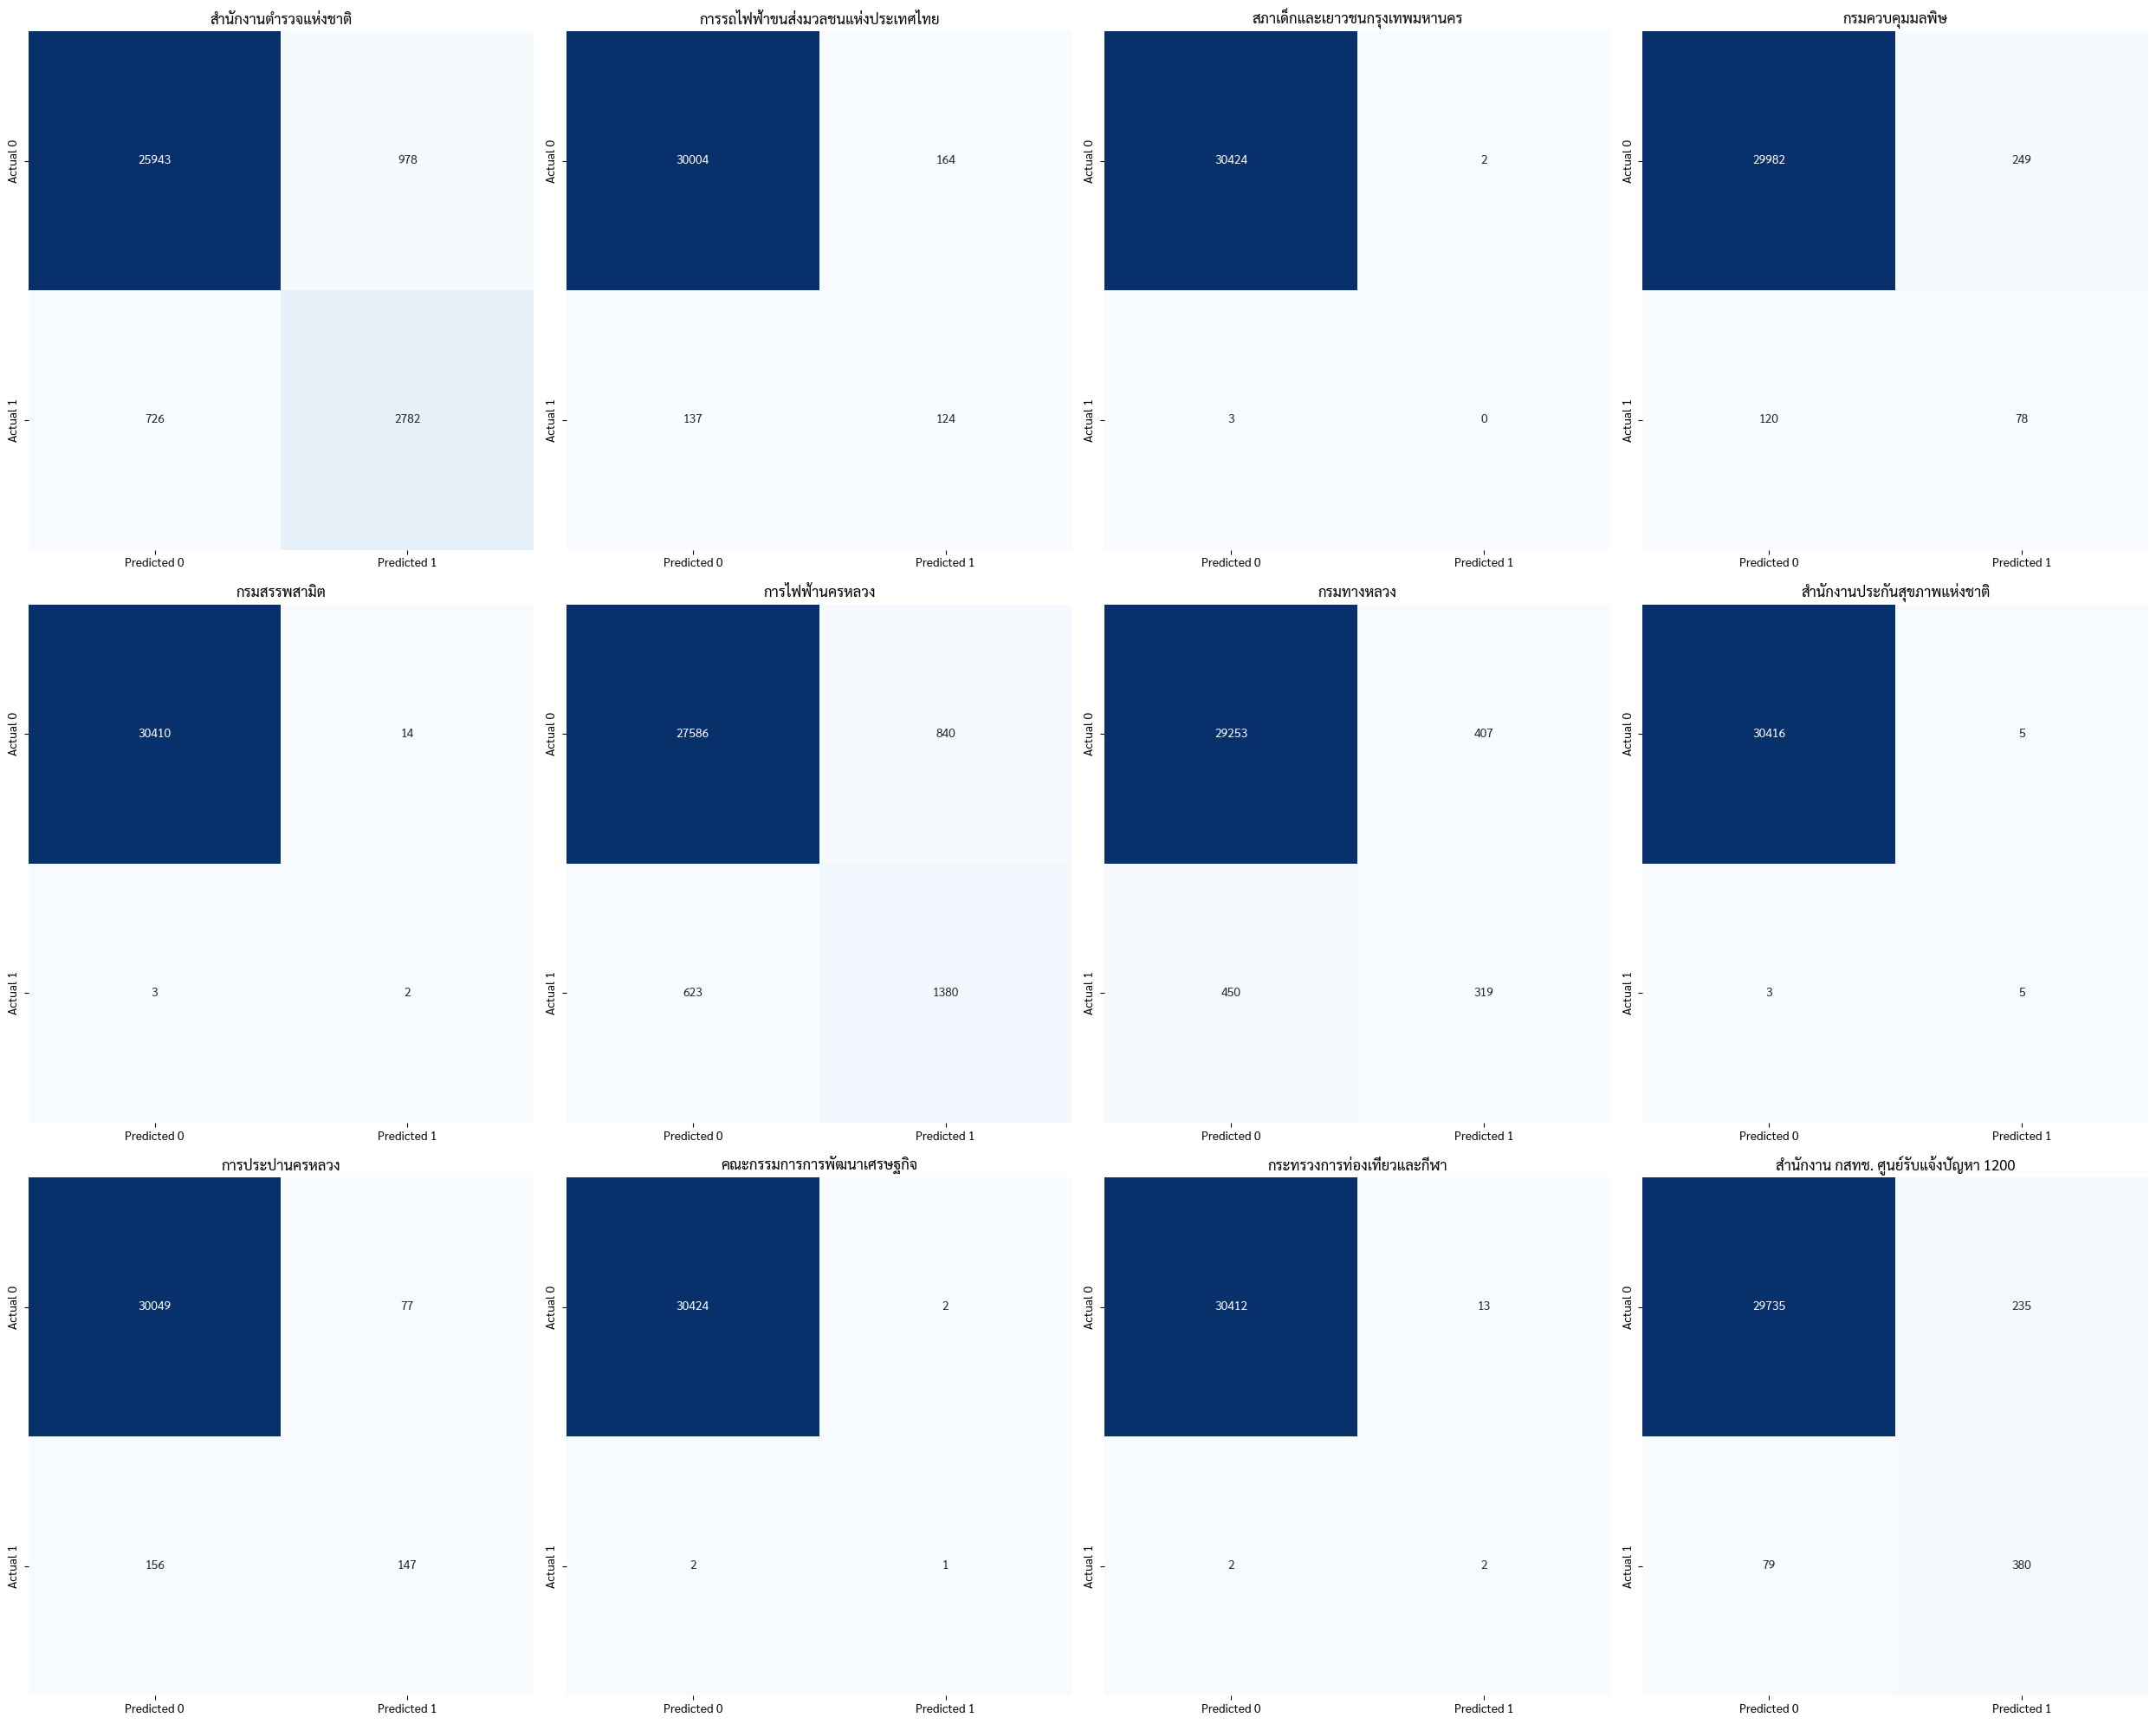
\includegraphics[width=\textwidth]{image_07}
                    \caption{Validation Confusion Matrix}
                \end{figure}

	\pagebreak

            \subsection{Classification Report}
                \begin{table}[h]
                \centering
                \begin{tabular}{|l|c|c|c|c|}
                    \hline
                    \rule{0pt}{2.5ex}
                    \textbf{Organization} & \textbf{Precision} & \textbf{Recall} & \textbf{F1 Score} & \textbf{Support} \\
                    \hline \hline
                    สำนักงานตำรวจแห่งชาติ & 0.74 & 0.79 & 0.77 & 3,508 \\
                    การรถไฟฟ้าขนส่งมวลชน & 0.43 & 0.48 & 0.45 & 201 \\
                    สภาเด็กและเยาวชน & 0.00 & 0.00 & 0.00 & 3 \\
                    กรมควบคุมมลพิษ & 0.24 & 0.39 & 0.30 & 198 \\
                    กรมสรรพสามิต & 0.12 & 0.40 & 0.19 & 5 \\
                    การไฟฟ้านครหลวง & 0.62 & 0.69 & 0.65 & 2,003 \\
                    กรมทางหลวง & 0.44 & 0.41 & 0.43 & 769 \\
                    สำนักงานประกันสุขภาพ & 0.50 & 0.62 & 0.56 & 8 \\
                    การประปานครหลวง & 0.66 & 0.49 & 0.56 & 303 \\
                    การพัฒนาเศรษฐกิจ & 0.33 & 0.33 & 0.33 & 3 \\
                    การท่องเที่ยวและกีฬา & 0.13 & 0.50 & 0.21 & 4 \\
                    สำนักงาน กสทช. & 0.62 & 0.83 & 0.71 & 459 \\
                    \hline \hline
                    \textbf{Type} & \textbf{Precision} & \textbf{Recall} & \textbf{F1 Score} & \textbf{Support} \\
                    \hline \hline
                    Micro Average & 0.64 & 0.69 & 0.66 & 7,524 \\
                    Macro Average & 0.40 & 0.49 & 0.43 & 7,524 \\
                    Weighted Average & 0.64 & 0.69 & 0.66 & 7,524 \\
                    Samples Average & 0.17 & 0.17 & 0.17 & 7,524 \\
                    \hline
                \end{tabular}
                \caption{Validation Classification Report}
            \end{table}

    \pagebreak

    \part{Result}

        \noindent The submission got 0.36637 Macro F1 Score on the public leaderboard
        \begin{figure}[h]
            \centering
            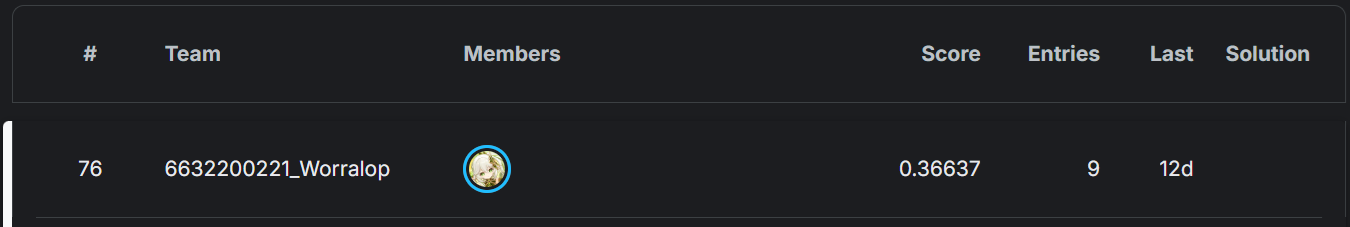
\includegraphics[width=\textwidth]{image_08}
            \caption{Public Leaderboard Result}
        \end{figure}

        \noindent The submission got 0.34254 Macro F1 Score on the private leaderboard
        \begin{figure}[h]
            \centering
            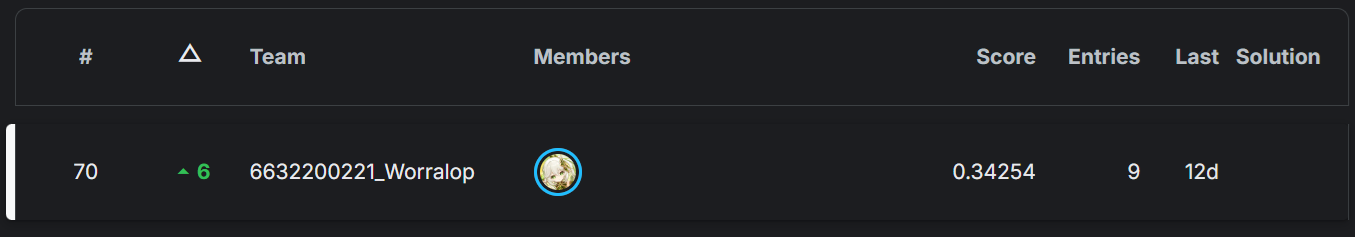
\includegraphics[width=\textwidth]{image_09}
            \caption{Private Leaderboard Result}
        \end{figure}

    \pagebreak

    \part{Discussion}
        \section{Problem \& Solution Analysis}
            \subsection{Problem}
                According to the dataset, it has several problems during the deep learning model implementation including
                \begin{itemize}
                    \item \textbf{Text Characters}: The raw dataset has lots of emojis and weird unicode characters
                    which decreased the efficiency of the model and wasted the computational resources.
                    \item \textbf{Non-Labeled Data}: About 76.01\% of the dataset are the non-labeled dataset.
                    Moreover, the topic of these data sometimes should be considered as labeled.
                    \item \textbf{Extreme Class Imbalance}: The dataset has only few rows for สำนักงานประกันสุขภาพแห่งชาติ
                    กรมสรรพสามิต กระทรวงการท่องเที่ยวและกีฬา สภาเด็กและเยาวชนกรุงเทพมหานคร and คณะกรรมการการพัฒนาเศรษฐกิจ (0.07\% of dataset in total).
                    This heavily affects the macro F1 score since it weights all classes equally.
                \end{itemize}

            \subsection{Solution}
                \noindent With those mentioned problems, we did implement some features to fix them.
                \begin{itemize}
                    \item \textbf{Text Cleaning}: All complaints text are thoroughly cleaned with punctuation, characters order,
                    spaces and remove all emojis and weird unicode characters. This improves the efficiency of the model.
                    \item \textbf{Positive Weight}: The positive weight is calculated to give more penalty to the model when
                    it predicts the minor classes wrong. This makes the model to actually learn to predict those classes
                    instead of dropping them which improves macro F1 score.
                \end{itemize}

        \section{Future Improvement}
            After successfully implementing this project, the author has thought the possible future improvement as follows:
            \begin{itemize}
                \item \textbf{Data Filtering}: In the project, the author did not filter out some of the unrelated report, such as
                \enquote{test ka}, \enquote{by traffy staff report for test \# traffywebsite \# english}.
                \item \textbf{Postprocessing}: The author has already performed the simple postprocessing by finding and matching a keyword
                then force change the prediction label. However, this method significantly decreases the score from 0.34254 to 0.23804.
                There might be more effective postprocessing method to improve the score.
                \item \textbf{Non-labeled Data}: As mentioned that the non-labeled is the majority of the dataset (76.01\%),
                training a model with all of them might not be a good idea. There might be more effective way to deal with this.
            \end{itemize}

    \pagebreak

    \part{Conclusion}
        In summary, the objective of this project is to design the data pipeline and implement a deep learning model to classify
        complaints text from Bangkok Traffy Fondue into the correct responsible government department.

        \vspace{1em}

        For the data cleaning, this project uses Python pandas to load raw CSV file as a DataFrame,
        then uses Python regex to find a pattern to remove or replace, and then uses PyThaiNLP to normalize
        and encode the Thai text.

        \vspace{1em}

        For the data pipeline, this project split the dataset into training dataset and validation dataset in 90:10 ratio
        by using iterative stratification method to ensure the equality of class ratio in both dataset.
        Next, we implement PyTorch DataModule to easily feed the data into a deep learning model as a batch.

        \vspace{1em}

        For the deep learning model, this project uses PhayaThaiBERT model for classification. We load the pre-trained model,
        set BCEWithLogitsLoss as a loss function and use Macro F1 score as an evaluation metric.
        In addition, we also use Adam optimizer with dynamic learning rate.

        \vspace{1em}

        For the fine-tuning process, this project dynamically adjust the probability threshold to convert logits score to class prediction
        for improving the validation macro F1 score.

        \vspace{1em}
        According to the validation result and submission result in Kaggle competition,
        this model reaches 0.36637 Macro F1 Score on the public leaderboard
        and 0.34254 Macro F1 Score on the private leaderboard which indicates that the model
        is still not performing well on the minor classes, but performing satisfactorily on the major classes.
        However, this model still needs improvement in the future as discussed in the discussion part.

\end{document}
